\documentclass[12pt,a4paper]{article}
\usepackage{amsmath,amscd,amsbsy,amssymb,latexsym,url,bm,amsthm}
\usepackage{epsfig,graphicx,subfigure}
\usepackage{enumitem,balance}
\usepackage{wrapfig}
\usepackage{mathrsfs,euscript}\usepackage{appendix}
\usepackage{soul}
\usepackage{listings}
\usepackage[usenames]{xcolor}
\usepackage{hyperref}
\usepackage[vlined,ruled,linesnumbered]{algorithm2e}
\usepackage{float}
\hypersetup{colorlinks=true,linkcolor=black}

\newtheorem{theorem}{Theorem}
\newtheorem{lemma}[theorem]{Lemma}
\newtheorem{proposition}[theorem]{Proposition}
\newtheorem{corollary}[theorem]{Corollary}
\newtheorem{exercise}{Exercise}
\newtheorem*{solution}{Solution}
\newtheorem{definition}{Definition}
\theoremstyle{definition}

\renewcommand{\thefootnote}{\fnsymbol{footnote}}

\newcommand{\postscript}[2]
{\setlength{\epsfxsize}{#2\hsize}
	\centerline{\epsfbox{#1}}}

\renewcommand{\baselinestretch}{1.0}

\setlength{\oddsidemargin}{-0.365in}
\setlength{\evensidemargin}{-0.365in}
\setlength{\topmargin}{-0.3in}
\setlength{\headheight}{0in}
\setlength{\headsep}{0in}
\setlength{\textheight}{10.1in}
\setlength{\textwidth}{7in}
\makeatletter \renewenvironment{proof}[1][Proof] {\par\pushQED{\qed}\normalfont\topsep6\p@\@plus6\p@\relax\trivlist\item[\hskip\labelsep\bfseries#1\@addpunct{.}]\ignorespaces}{\popQED\endtrivlist\@endpefalse} \makeatother
\makeatletter
\renewenvironment{solution}[1][Solution] {\par\pushQED{\qed}\normalfont\topsep6\p@\@plus6\p@\relax\trivlist\item[\hskip\labelsep\bfseries#1\@addpunct{.}]\ignorespaces}{\popQED\endtrivlist\@endpefalse} \makeatother

\begin{document}
	\noindent
	
	%========================================================================
	\noindent\framebox[\linewidth]{\shortstack[c]{
			\Large{\textbf{Lab05-DynamicProgramming}}\vspace{1mm}\\
			CS214-Algorithm and Complexity, Xiaofeng Gao, Spring 2021.}}
\begin{center}
\footnotesize{\color{blue}$*$ Name:\underline{\quad   Haoyi You  \quad  }\quad Student ID:\underline{\quad 519030910193 \quad} \quad Email: \underline{\quad yuri-you@sjtu.edu.cn \quad}}
\end{center}
	
	\begin{enumerate}
		\item \textit{Optimal Binary Search Tree.} Given a sorted sequence $K=\left \langle k_{1}, k_{2}, \ldots, k_{n} \right \rangle$ of $n$ distinct keys, and we wish to build a binary search tree from these keys. For each key $k_{i}$, we have a probability $p_{i}$ that a search will be for $k_{i}$. Some searches may be for values not in $K,$ and so we also have $n+1$ \emph{dummy keys} $d_{0}, d_{1}, d_{2}, \ldots, d_{n}$ representing values not in $K$. In particular, $d_{0}$ represents all values less than $k_{1}$, and $d_{n}$ represents all values greater than $k_{n}$. For $i=1,2, \ldots, n-1,$ the dummy key $d_{i}$ represents all values between $k_{i}$ and $k_{i+1}$. For each dummy key $d_{i}$, we have a probability $q_{i}$ that a search will correspond to $d_{i}$. Each key $k_{i}$ is an internal node, and each dummy key $d_{i}$ is a leaf. Every search is either successful (finding some key $k_{i}$ ) or unsuccessful (finding some dummy key $d_{i}$ ), and so we have $ \sum_{i=1}^{n} p_{i}+\sum_{i=0}^{n} q_{i}=1 $. 
		\begin{enumerate}
			\item Prove that if an optimal binary search tree $T$ ($ T $ has the smallest expected search cost) has a subtree $T^{\prime}$ containing keys $k_{i}, \ldots, k_{j},$ then this subtree $T^{\prime}$ must be optimal as well for the subproblem with keys $k_{i}, \ldots, k_{j}$ and dummy keys $d_{i-1}, \ldots, d_{j}$. 
			\item We define $e[i, j]$ as the expected cost of searching an optimal binary search tree containing the keys $k_{i}, \ldots, k_{j} .$ Our goal is to compute $e[1, n]$. Write the state transition equation and pseudocode using \textbf{dynamic programming} to find
			the minimum expected cost of a search in a given binary tree. (\textbf{Remark}: You may use $ w(i, j)=\sum_{l=i}^{j} p_{l}+\sum_{l=i-1}^{j} q_{l} $).
			\item Implement your proposed algorithm in C/C++ and analyze the time complexity. ({\color{blue}The framework Code-OBST.cpp is attached on the course webpage}). Give the minimum search cost calculated by your algorithm. The test case is given as following:
			\begin{table}[H]
				\setlength{\abovecaptionskip}{0cm}
				\setlength{\belowcaptionskip}{0.1cm}
				\centering		
				\begin{tabular}{|c|cccccccc|}
					\hline
					$ i $&0&1&2&3&4&5&6&7\\
					\hline
					$ p_{i} $&&0.04&0.06&0.08&0.02&0.10&0.12&0.14\\
					\hline
					$ q_{i} $&0.06&0.06&0.06&0.06&0.05&0.05&0.05&0.05\\
					\hline
				\end{tabular}
			\end{table}
			\item Please draw the structure of the optimal binary search tree in the test case, and explain the drawing process.   
		\end{enumerate}
		    \begin{solution}
		    ~\par
		       \begin{enumerate}
		           \item We assume the depth of $k_i$ is $h_i$,and depth of $d_i$ is $g_i$. Let depth of the root of $T^{\prime}$ is $h$. If $T^{\prime}$ is not optimal(depth of the node (in $T^\prime) $is $h_{i}-h, \ldots, h_{j}-h$),there exists another optimal solution $T^{\prime\prime}$(depth of the node is $h_{i}^{\prime}-h, \ldots, h_{j}^{\prime}-h$). So we build another tree $S$ with $\forall$ node $k\in S$,if $k\in T^\prime,h(S)_k=h_{k}^{\prime}$,else $h(S)_k=h_{i}^\prime$.\\
		           $ Cost_T-Cost_S=(h_{i}-h_{i}^{\prime})*p_i\ldots(h_{j}-h_{j}^{\prime})*p_j>0$,so $T$ is not optimal.
		           \item~\par
		           \begin{algorithm}[H]
                    \KwIn{probability array \{$p_1,p_2\dots p_n$\} and probability array \{$q_0,q_1\dots q_n$\}}
                    \KwOut{minimum expected cost C}
        		 \BlankLine
        \caption{Optimal Binary Search Tree}
        \label{algorithm}
        % $quicksort(data)$\\
        % Initialize $Answer[k]$\\
        % \For{$i = 1 \text{ to } k$ }{
        %   $Answer[i]\leftarrow data[i]$
        % }
        % \Return $Answer$\;\\
       $e[n][n]\leftarrow0$;\\
       $w[n][n]\leftarrow0$;\\
       \For{$i = 0 \text{ to } n-1$}{
        $w[i][i]\leftarrow p_{i+1}+q_{i}+q_{i+1}$;//array index begins at 0\\
       }
       \For{$i = 1 \text{ to } n-1$}{
        \For{$j = 0 \text{ to } n-1-i$}{
            $w[j][j+i]\leftarrow w[j][j+i-1]+p_{j+i+1}+q_{j+i+1}$;\\
        }
       }
        \For{$i = 0 \text{ to } n-1$ }{
             \For{$j = 0 \text{ to } n-i-1$ }{
                  \For{$k = 0 \text{ to } i$}{
                    \If{k == 0}{
                    $left\leftarrow2*q_j$;//left subtree is a leaf\\
                    }
                    \Else{
                    $left\leftarrow e[j-1][j+k-1]+w[j-1][j+k-1]$;\\
                    }
                    \If{k==i}{
                    $right\leftarrow2*q_{j+i+1}$;//right subtree is a leaf\\
                    }
                    \Else{
                    $right\leftarrow e[j+1+k][j+i-1]+w[j+1+k][j+i-1]$;\\
                    }
                    $sum\leftarrow left+right+p_{j+k}$;\\
                \If{$sum>e[j][j+i]$}{
                $e[j][j+i]\leftarrow sum$;\\
                }
              }
              }
         }
        \Return $e[0][n-1]$;
        \end{algorithm}
        \item the answer is 3.12,the code is in the appendix and for the result result please refer to Figure~\ref{OBST} 

        \item
        The structure is in Figure~\ref{OBST}. You can also refer to Figure~\ref{OBST1}\\
        The drawing process is a recursive process using algorithm DFS. Firstly we find the root of the whole tree,assuming as $k$. Then we would do this recursively to the left subtree and right subtree of this tree,that is to do this $[1,k-1]$ and $[k+1,n]$.\\
        The whole process rely to a recursive function $void~construct\_optimal\_bst(int~i, int~j)$
        \begin{figure}[htbp]
        \centering
        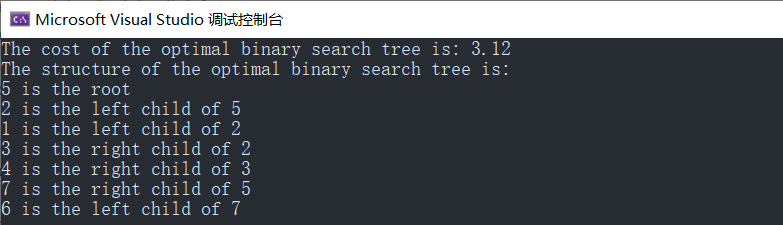
\includegraphics[width=0.8\textwidth]{OBST.png}
        \caption{OBST result}\label{OBST}
        \end{figure}
        \begin{figure}[htbp]
        \centering
        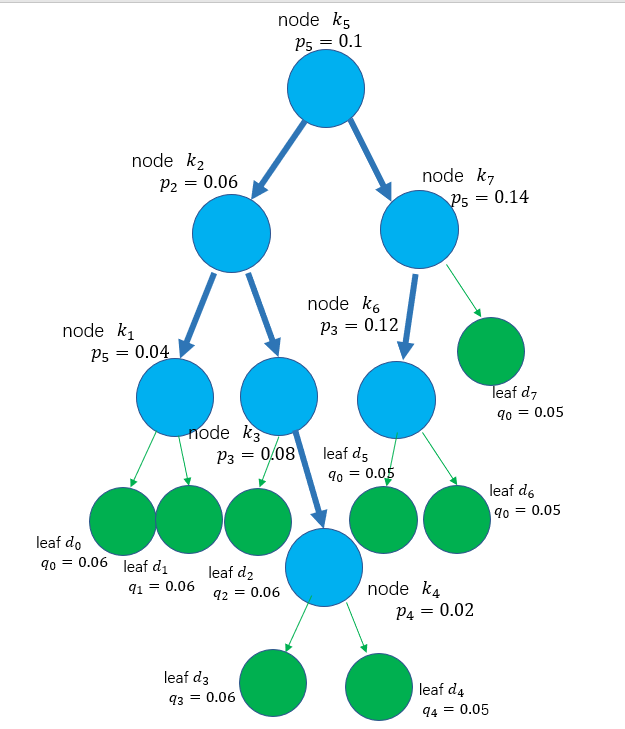
\includegraphics[width=0.8\textwidth]{OBST1.png}
        \caption{OBST structure}\label{OBST1}
        \end{figure}
		\end{enumerate}
		\end{solution}
		
		\item \textit{Dynamic Time Warping Distance.} \textbf{DTW} stretches the series along the time axis in a dynamic way over different
		portions to enable more effective matching. Let $D T W(i, j)$ be the optimal distance between the first $i$ and first $j$ elements of two time series $\bar{X}=\left(x_{1} \ldots x_{n}\right)$ and $\bar{Y}=\left(y_{1} \ldots y_{m}\right),$ respectively. Note that the two time series are of lengths $n$ and $m$, which may not be the same. Then, the value of $D T W(i, j)$ is defined recursively as follows:
		$$
		DTW(i, j)=\left|x_{i}- y_{j}\right|+\min(DTW(i, j-1), DTW(i-1, j), DTW(i-1, j-1))
		$$
		
		\begin{enumerate}
			\item Implement the proposed DTW algorithm in C/C++ and analyze the time complexity of your implementation. ({\color{blue}The framework Code-DTW.cpp is attached on the course webpage}). Two test cases have been given in the source code. 
			\item The window constraint imposes a minimum level $w$ of positional alignment between matched elements. The window constraint requires that $DTW(i, j)$ be computed only when $|i-j| \leq w$. Modify your code to add a window constraint and give the results of $ w=0 $ and $ w=1 $ on the two test cases. 
		\end{enumerate}
		    \begin{solution}
		    \begin{enumerate}
		        \item The answer is 0 and 1.25.Please refer to \ref{DTW1} for more details.
		        \item The answer is 7.8 and 1.9.Please refer to \ref{DTW2} for more details.
		    \end{enumerate}
        \begin{figure}[htbp]
        \centering
        
\includegraphics[width=0.8\textwidth]{DTW1.png}
        \caption{DTW result}\label{DTW1}
        \end{figure}
        \begin{figure}[htbp]
        \centering
        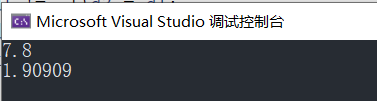
\includegraphics[width=0.8\textwidth]{DTW2.png}
        \caption{DTW structure}\label{DTW2}
        \end{figure}
		    \end{solution}
		
	\end{enumerate}
	
\vspace{20pt}
\appendix
\section{Appendix1}
\begin{lstlisting}[language=C++]
#include <iostream>
using namespace std;
#define MAX 10000
const int n = 7;
double p[n + 1] = {0,0.04,0.06,0.08,0.02,0.10,0.12,0.14};
double q[n + 1] = {0.06,0.06,0.06,0.06,0.05,0.05,0.05,0.05};
int root[n + 1][n + 1];
double e[n + 2][n + 2] = { 0 };
double w[n + 2][n + 2] = { 0 };
void optimal_binary_search_tree(double *p,double *q,int n)
{   
    for (int i = 1; i <= n; ++i) {
        w[i][i] = p[i] + q[i - 1] + q[i];
    }
    for (int i = 1; i <=n; ++i) {
        for (int j = 1; j <= n - i; ++j) {
            w[j][i + j] = w[j][j + i - 1] + p[j + i] + q[j + i];
        }
    }
    for (int i = 1; i <= n; ++i) {
        for (int j = 1; j <= n - i+1; ++j) {
            for (int k = 1; k <= i; ++k) {
                double left, right;
                if (k == 1) {
                    left = 2 * q[j - 1];
                }
                else {
                    left = e[j][j + k-2] + w[j][j + k-2];
                }
                if (k == i) {
                    right = 2 * q[j + i-1];
                }
                else {
                    right = e[j + k][j + i - 1] + w[j + k][j + i - 1];
                }
                
                double sum = left + right + p[j + k - 1];
                if (e[j][i + j - 1] == 0||e[j][i + j - 1] > sum) {
                    e[j][i + j - 1] = sum;
                    root[j][i + j - 1] = j + k - 1;
                }
            }
        }
    }

}

void construct_optimal_bst(int i, int j)
{
    if (i == 1 && j == n) {
        cout << root[1][n] << " is the root\n";
    }
    int root1 = root[i][j];
    if (root1 != i) {
        cout << root[i][root1 - 1] << "is the left child of" << root1 << endl;
        construct_optimal_bst(i, root1 - 1);
    }
    if (root1 != j) {
        cout<<root[root1+1][j]<< " is the right child of " << root1 << endl;
        construct_optimal_bst(root1 + 1,j);
    }
}
/*
Please write your code here.
*/


int main()
{
    optimal_binary_search_tree(p,q,n);
    cout<<"The cost of the optimal binary search tree is: "<<e[1][n]<<endl;
    cout << "The structure of the optimal binary search tree is: " << endl;
    construct_optimal_bst(1,n);
    return 0;
}


\end{lstlisting}
\section{Appendix2}
\begin{lstlisting}[language=C++]
#include <iostream>
#include <vector>
#include <cmath>
#include <numeric>
/*
The process to calculate the dynamic can be divided into four steps:
1.Create an empty cost matrix DTW with X and Y labels as amplitudes of the two series to be compared.
2.Use the given state transition function to fill in the cost matrix.
3.Identify the warping path starting from top right corner of the matrix and traversing to bottom left. The traversal path is identified based on the neighbor with minimum value.
i.e., When we reach the point (i, j) in the matrix, the next position is to choose the point with the smallest cost among (i-1,j-1), (i,j-1), and (i-1,j),
For the sake of simplicity, when the cost is equal, the priority of the selection is (i-1,j-1), (i,j-1), and (i-1,j) in order.
4.Calculate th time normalized distance. We define it as the average cost of the selected points.
*/
using namespace std;
void warp_path(const vector<vector<int>>& data, vector<int>& ans, int n, int m) {
    if (n == 0) {
        if (m != 0)warp_path(data, ans, n, m - 1);
    }
    else {
        if (m == 0)warp_path(data, ans, n - 1, m);
        else {
            int min = data[n - 1][m - 1];
            if (min > data[n - 1][m])min = data[n - 1][m];
            if (min > data[n][m - 1])min = data[n][m - 1];
            if (min == data[n - 1][m - 1])warp_path(data, ans, n - 1, m - 1);
            else {
                if(min==data[n][m-1])warp_path(data, ans, n, m - 1);
                else {
                    warp_path(data, ans, n-1, m);
                }
            }
        }
    }
    ans.push_back(data[n][m]);
}
double distance(vector<int> x, vector<int> y) {
    int n = x.size();
    int m = y.size();
    vector<vector<int>> DTW;
    //Use the given state transition function to fill in the cost matrix.
    /*
    Please write your code here.
    
    */
    for (int i = 0; i < n; ++i) {
        DTW.push_back(vector<int>());
        for (int j = 0; j < n; ++j) {
            int d1, d2, d3;
            if (i == 0) {
                if (j == 0) {
                    d1 = d2 = d3 = 0;
                }
                else {
                    d2 = DTW[i][j - 1];
                    d1 = d3 = d2+1;
                }
            }
            else {
                if (j == 0) {
                    d1 = DTW[i - 1][j];
                    d2 = d3 = d1+1;
                }
                else {
                    d1 = DTW[i - 1][j];
                    d2 = DTW[i][j - 1];
                    d3 = DTW[i-1][j - 1];
                }
            }
            if (d2 < d1)d1 = d2;
            if (d3 < d1)d1 = d3;
            DTW[i].push_back(d1 + abs(x[i] - y[j]));
        }
    }
    vector<int> d;
    warp_path(DTW, d, n-1, m-1);
    //Identify the warping path.
    /*
    Please write your code here.
    */

    double ans = 0;
    ans = double(DTW[n-1][m-1]) / d.size();
    //Calculate th time normalized distance
    /*
    Please write your code here.
    */
    return ans;
}

int main(){
	vector<int> X,Y;
	//test case 1
	X = {37,37,38,42,25,21,22,33,27,19,31,21,44,46,28};
	Y = {37,38,42,25,21,22,33,27,19,31,21,44,46,28,28};
	cout<<distance(X,Y)<<endl;
	//test case 2
	X = {11,14,15,20,19,13,12,16,18,14};
	Y = {11,17,13,14,11,20,15,14,17,14};
	cout<<distance(X,Y)<<endl;
	//Remark: when you modify the code to add the window constraint, the distance function has thus three inputs: X, Y, and the size of window w.
	return 0;
}
\section{Appendix1}
\begin{lstlisting}[language=C++]
#include <iostream>
using namespace std;
#define MAX 10000
const int n = 7;
double p[n + 1] = {0,0.04,0.06,0.08,0.02,0.10,0.12,0.14};
double q[n + 1] = {0.06,0.06,0.06,0.06,0.05,0.05,0.05,0.05};
int root[n + 1][n + 1];
double e[n + 2][n + 2] = { 0 };
double w[n + 2][n + 2] = { 0 };
void optimal_binary_search_tree(double *p,double *q,int n)
{   
    for (int i = 1; i <= n; ++i) {
        w[i][i] = p[i] + q[i - 1] + q[i];
    }
    for (int i = 1; i <=n; ++i) {
        for (int j = 1; j <= n - i; ++j) {
            w[j][i + j] = w[j][j + i - 1] + p[j + i] + q[j + i];
        }
    }
    for (int i = 1; i <= n; ++i) {
        for (int j = 1; j <= n - i+1; ++j) {
            for (int k = 1; k <= i; ++k) {
                double left, right;
                if (k == 1) {
                    left = 2 * q[j - 1];
                }
                else {
                    left = e[j][j + k-2] + w[j][j + k-2];
                }
                if (k == i) {
                    right = 2 * q[j + i-1];
                }
                else {
                    right = e[j + k][j + i - 1] + w[j + k][j + i - 1];
                }
                
                double sum = left + right + p[j + k - 1];
                if (e[j][i + j - 1] == 0||e[j][i + j - 1] > sum) {
                    e[j][i + j - 1] = sum;
                    root[j][i + j - 1] = j + k - 1;
                }
            }
        }
    }

}

void construct_optimal_bst(int i, int j)
{
    if (i == 1 && j == n) {
        cout << root[1][n] << " is the root\n";
    }
    int root1 = root[i][j];
    if (root1 != i) {
        cout << root[i][root1 - 1] << "is the left child of" << root1 << endl;
        construct_optimal_bst(i, root1 - 1);
    }
    if (root1 != j) {
        cout<<root[root1+1][j]<< " is the right child of " << root1 << endl;
        construct_optimal_bst(root1 + 1,j);
    }
}
/*
Please write your code here.
*/


int main()
{
    optimal_binary_search_tree(p,q,n);
    cout<<"The cost of the optimal binary search tree is: "<<e[1][n]<<endl;
    cout << "The structure of the optimal binary search tree is: " << endl;
    construct_optimal_bst(1,n);
    return 0;
}


\end{lstlisting}
\section{Appendix3}
\begin{lstlisting}[language=C++]
#include <iostream>
#include <vector>
#include <cmath>
#include <numeric>
/*
The process to calculate the dynamic can be divided into four steps:
1.Create an empty cost matrix DTW with X and Y labels as amplitudes of the two series to be compared.
2.Use the given state transition function to fill in the cost matrix.
3.Identify the warping path starting from top right corner of the matrix and traversing to bottom left. The traversal path is identified based on the neighbor with minimum value.
i.e., When we reach the point (i, j) in the matrix, the next position is to choose the point with the smallest cost among (i-1,j-1), (i,j-1), and (i-1,j),
For the sake of simplicity, when the cost is equal, the priority of the selection is (i-1,j-1), (i,j-1), and (i-1,j) in order.
4.Calculate th time normalized distance. We define it as the average cost of the selected points.
*/
using namespace std;
void warp_path(const vector<vector<int>>& data, vector<int>& ans, int n, int m,int constrain) {
    if (n == 0) {
        if (m != 0)warp_path(data, ans, n, m - 1, constrain);
    }
    else {
        if (m == 0)warp_path(data, ans, n - 1, m, constrain);
        else {
            int min = data[n - 1][m - 1];
            if (min > data[n - 1][m]&&abs(n-1-m)<=constrain)min = data[n - 1][m];
            if (min > data[n][m - 1] && abs(m - 1 - n) <= constrain)min = data[n][m - 1];
            if (min == data[n - 1][m - 1])warp_path(data, ans, n - 1, m - 1, constrain);
            else {
                if(min==data[n][m-1])warp_path(data, ans, n, m - 1, constrain);
                else {
                    warp_path(data, ans, n-1, m, constrain);
                }
            }
        }
    }
    ans.push_back(data[n][m]);
}
double distance(vector<int> x, vector<int> y,int window_constrain) {
    int n = x.size();
    int m = y.size();
    vector<vector<int>> DTW;
    //Use the given state transition function to fill in the cost matrix.
    /*
    Please write your code here.
    
    */
    for (int i = 0; i < n; ++i) {
        DTW.push_back(vector<int>());
        for (int j = 0; j < n; ++j) {
            if (abs(i - j) > window_constrain) {
                DTW[i].push_back(-1);
                continue;
            }
            int d1, d2, d3;
            if (i == 0) {
                if (j == 0) {
                    d1 = d2 = d3 = 0;
                }
                else {
                    d2 = DTW[i][j - 1];
                    d1 = d3 = -1;
                }
            }
            else {
                if (j == 0) {
                    d1 = DTW[i - 1][j];
                    d2 = d3 = -1;
                }
                else {
                    d1 = DTW[i - 1][j];
                    d2 = DTW[i][j - 1];
                    d3 = DTW[i - 1][j - 1];
                }
            }
            if (d3 == -1) {
                if (d2 != -1)d3 = d2 + 1;
                else d3 = d1 + 1;
            }
            if (d1 < d3 && d1 != -1)d3 = d1;
            if (d2 < d3 && d2 != -1)d3 = d2;
            DTW[i].push_back(d3 + abs(x[i] - y[j]));
        }
    }
    vector<int> d;
    warp_path(DTW, d, n-1, m-1,window_constrain);
    //Identify the warping path.
    /*
    Please write your code here.
    */

    double ans = 0;
    ans = double(DTW[n-1][m-1]) / d.size();
    //Calculate th time normalized distance
    /*
    Please write your code here.
    */
    return ans;
}

int main(){
	vector<int> X,Y;
	//test case 1
	X = {37,37,38,42,25,21,22,33,27,19,31,21,44,46,28};
	Y = {37,38,42,25,21,22,33,27,19,31,21,44,46,28,28};
    X1 = X, Y1 = Y;
	cout<<distance(X,Y,0)<<endl;
	//test case 2
	X = {11,14,15,20,19,13,12,16,18,14};
	Y = {11,17,13,14,11,20,15,14,17,14};
    X1 = X, Y1 = Y;
	cout<<distance(X,Y,1)<<endl;
	//Remark: when you modify the code to add the window constraint, the distance function has thus three inputs: X, Y, and the size of window w.
	return 0;
}



\end{lstlisting}	
	%========================================================================
\end{document}
